\section{Tokens}

\begin{defi}{Token-basierte Authentifikation}
    Bei der \emph{Token-basierten Authentifizierung} handelt es sich um ein Protokoll, das es den Nutzenden ermöglicht, ihre Identität zu verifizieren und im Gegenzug ein eindeutiges Zugangstoken zu erhalten.

    Während der Gültigkeitsdauer des Tokens können die Nutzenden dann auf die Website oder Anwendung zugreifen, für die das Token ausgestellt wurde.

    Sie müssen ihre Anmeldedaten nicht jedes Mal neu eingeben, wenn sie dieselbe Website, Anwendung oder eine andere mit demselben Token geschützte Ressource aufrufen.
\end{defi}

\begin{defi}{OAuth 2.0}
    \emph{OAuth} ist der Name zweier verschiedener offener Protokolle, die eine standardisierte, sichere API-Autorisierung für Desktop-, Web- und Mobile-Anwendungen erlauben.
    OAuth 1.0 wurde ab 2006 entwickelt und 2007 veröffentlicht.
    OAuth 2.0, das sich grundlegend von OAuth 1.0 unterscheidet, wurde 2012 veröffentlicht.

    Typischerweise wird dabei die Übermittlung von Passwörtern an Dritte vermieden.

    Auf Basis von OAuth 2.0 wird OpenID Connect heute in vielen Internetdiensten auch zur Authentifizierung von Benutzern eingesetzt.

    In OAuth 2.0 existieren vier Rollen:
    \begin{itemize}
        \item \emph{Resource Owner}:
              \begin{itemize}
                  \item Eine Entität (\emph{User}), die einem Dritten den Zugriff auf ihre geschützten Ressourcen gewähren kann.
                  \item Diese Ressourcen werden durch den \emph{Resource Server} bereitgestellt.
                  \item Ist der Resource Owner eine Person, wird dieser als User bezeichnet.
              \end{itemize}
        \item \emph{Resource Server}:
              \begin{itemize}
                  \item Der Server (\emph{Dienst}), auf dem die geschützten Ressourcen (\emph{Protected Resources}) liegen.
                  \item Er ist in der Lage, auf Basis von \emph{Access Tokens} darauf Zugriff zu gewähren.
                  \item Ein solcher Token repräsentiert die delegierte \emph{Autorisierung des Resource Owners}.
              \end{itemize}
        \item \emph{Client}:
              \begin{itemize}
                  \item Eine Anwendung (\emph{Relying Party}), die auf geschützte Ressourcen des Resource Owners zugreifen möchte, die vom Resource Server bereitgestellt werden.
                  \item Der Client kann auf einem Server (Webanwendung), Desktop-PC, mobilen Gerät etc. ausgeführt werden.
              \end{itemize}
        \item \emph{Authorization Server}:
              \begin{itemize}
                  \item Der Server authentifiziert den Resource Owner und stellt Access-Tokens für den vom Resource Owner erlaubten Anwendungsbereich (\emph{Scope}) aus.
                  \item Authorization Server und Resource Server werden häufig zusammengelegt und gemeinsam betrieben.
              \end{itemize}
    \end{itemize}
\end{defi}

\begin{bonus}{OAuth 2.0 Protokollfluss}
    \centering
    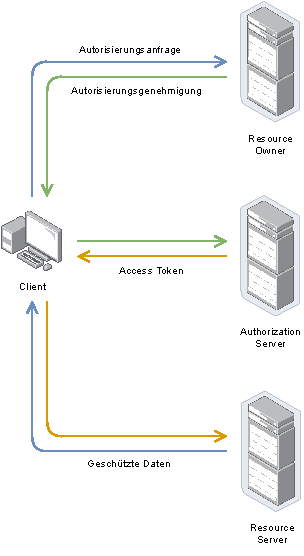
\includegraphics[width=.4\textwidth]{includes/figures/bonus_oauth2.pdf}
\end{bonus}

\begin{defi}{JSON Web Token}
    Ein \emph{JSON Web Token} ist ein auf JSON basiertes Access-Token.

    Das JWT ermöglicht den Austausch von verifizierbaren \emph{Claims}.

    Es wird typischerweise verwendet, um in einem System mit einem Drittanbieter die Identität eines Benutzers zwischen einem Identity-Provider und einem Service-Provider auszutauschen.

    JWT eignen sich vor allem zur Implementierung von \emph{Stateless Sessions}, da sämtliche authentifizierungsrelevanten Informationen im Token übertragen werden können und die Sitzung nicht zusätzlich auf einem Server gespeichert werden muss.

    Ein JWT besteht aus drei Teilen: dem Header, Payload und der Signatur.

    Der \emph{Header} ist ein JSON-Element, welches beschreibt, um welchen Token-Typ es sich handelt und welche Verschlüsselungsmethode zum Einsatz kommt.:

    \begin{tabularx}{\textwidth}{|l|l|X|}
        \hline
        Feld         & Name         & Bedeutung                                                                                                                                                               \\
        \hline
        \hline
        \texttt{typ} & Type         & Beschreibt den IANA Medientyp des Tokens. Dieser Wert ist immer JWT, um den Medientyp application/jwt zu beschreiben.                                                   \\
        \hline
        \texttt{cty} & Content Type & Dieses Feld wird benötigt, wenn das JWT ein anderes JWT als Payload enthält. In diesem Fall wird es auf JWT gesetzt. Andernfalls sollte dieses Feld weggelassen werden. \\
        \hline
        \texttt{alg} & Algorithm    & Beschreibt, welche Signaturmethode zum Einsatz kommt.                                                                                                                   \\
        \hline
    \end{tabularx}

    Beim \emph{Payload} handelt es sich um ein JSON-Element, welches die Claims beschreibt.

    Die \emph{Signatur} wird dadurch erzeugt, dass der Header und der Payload im Base64 kodierten und durch einen Punkt getrennten Format mit der spezifizierten Hashmethode gehasht wird.
\end{defi}

\begin{bonus}{OpenID und OpenID Connect}
    \emph{OpenID} ist ein dezentrales Authentifizierungssystem für webbasierte Dienste.

    Es erlaubt einem Client, der sich bei seinem OpenID-Provider einmal mit Benutzername und Kennwort angemeldet hat, sich mithilfe der OpenID (einer URL, in diesem Kontext auch Identifier genannt) ohne Benutzername und Passwort bei allen das System unterstützenden Websites – den Relying Parties – anzumelden, wendet also das \emph{Single-Sign-on-Prinzip} an.

    \emph{OpenID Connect (OIDC)} ist eine Authentifizierungsschicht, die auf dem Autorisierungsframework OAuth 2.0 basiert.
\end{bonus}

\begin{bonus}{ID-Token}
    Ein \emph{ID-Token} ist ein Artefakt, das beweist, dass ein Client authentifiziert wurde.

    Ein ID-Token ist als JSON-Web-Token (JWT) kodiert mit dem eine Anwendung den Inhalt leicht überprüfen und sicherstellen kann, dass er vom erwarteten Aussteller stammt und nicht von jemand anderem geändert wurde.
\end{bonus}

\begin{bonus}{Access-Token}
    Im OAuth 2.0-Kontext ermöglicht ein \emph{Access-Token} einer Client-Anwendung den Zugriff auf eine bestimmte Ressource, um bestimmte Aktionen im Namen eines Benutzers durchzuführen.

    Dies ist ein sogenanntes \emph{delegiertes Autorisierungsszenario}:
    Der User delegiert eine Client-Anwendung, um in seinem Namen auf eine Ressource zuzugreifen.
\end{bonus}